Let $\tset\in \Top$ be compact and locally of singular shape with
associated space $\ani{\tset}$.
Given some self map
$f\colon\tset\to\tset$, we can now associated two different invariants
to this datum, namely the Lefschetz character
\[ \lambda^f\colon \cptSections{\tset^f;\SS}\to \SS\,,\]
as well as the Reidemeister character 
\[ \rho_{f}\colon \SS \to \SS [\cL^{f}\ani{\tset}]\,,\]
of the induced map on spaces
map $f\colon \ani{\tset}\to \ani{\tset}$.

\begin{defn}\label{defn: Nielsen number}
   The rationalization of the Reidemeister character provides
   a class 
   \[[\rho_f]_{\QQ}\in \pi_0\QQ[\cL^f\ani{\tset}] \simeq
   \QQ[\pi_0\cL^f\ani{\tset}]\,.\]
   We define the \tdef{Nielsen Number} of $f$ denoted $\mdef{N_f}$ to be the support of $[\rho_f]_{\QQ}$ in
   this basis.
\end{defn}

Note under these assumptions on $f$ and $X$ we have that 
$\cptSections{\tset^f;\SS}^{\vee}\simeq \Sections{\tset^f;\omega_{\tset^f}} \simeq \SS[\ani{\tset^f}]$, and hence we can 
consider the dual of $\lambda^f$ as map of spectra
\[ \lambda_f\colon \SS \to \SS[\ani{\tset^f}]\,.\]
Moreover, there is a natural assembly map $\ass\colon \SS[\ani{\tset^f}]\to \SS[\cL^f\ani{\tset}]$ induced
by taking an actual fixed point $x\in \tset$ to the
constant path $x\to x$. The goal of this section is
to prove the following compatibility of these constructions:

\begin{thm}\label{thm: lefschetz-nielsen}
    Let $\tset \in \Top$ be compact and locally of singular shape. 
    Then we have a commutative diagram in the category of spectra:
    \[\begin{tikzcd}
	& {\Sections{\tset^f,\omega_{\tset}}} \\
	\SS & {\SS[\cL^f\ani{\tset}]}
	\arrow["{\mathfrak{a}}", from=1-2, to=2-2]
	\arrow["{\lambda_f}", from=2-1, to=1-2]
	\arrow["{\rho_f}"', from=2-1, to=2-2]
\end{tikzcd}\]
which is natural in intertwining maps.
\end{thm}

This immediately implies:

\begin{cor}
   Let $X\in \Top$ be compact of singular shape and let
   $f\colon X\to X$ be a self map. For any map $g\colon X\to X$
   that is homotopic to $f$ we have that
   \[ \#X^g \geq N_f\,.\]
\end{cor}

 We prove this by following the pattern of~\cref{sec: lefschetz theory}. First, then, we factor the square
\begin{equation}
  \label{eq:lax-comm-square-reidemeister}
  \begin{tikzcd}[column sep=large]
    \Sp \arrow[r,"\ani{\tset}^*"] \arrow[d,equal] & \Sp^{\ani{\tset}} \arrow[d,"g^*"]\\
    \Sp \arrow[r,swap,"\ani{\tset} ^*"] & \Sp^{\ani{\tset}}
  \end{tikzcd}
\end{equation}

through an object in $\Endtrl(\Prlstf)$ that has access to actual topological information about the pair $(\tset,f)$. Such a factorization is achieved by the {\em assembly functor} of Bartels and Nikolaus. Although this work is the subject of a still unpublished article, an expository account can be found in the lecture notes~\cite{Nikolaus2024}.

\subsection{Cosheaves and assembly}

\begin{defn}[Bartels--Nikolaus]\label{defn: abstract assembly}
  Let $(\mathcal C,\otimes ,\1)$ be a closed symmetric monoidal category with internal mapping object $\Hom_{\mathcal C}({-},{-})$. Given objects $A$ and $B$ in $\mathcal C$ together with a map 
  \[
    \delta\colon \1\to A\otimes B,
  \]
  the associated {\em $\delta$-assembly map}, denoted $a_\delta$, is defined by the following string diagram 
  \begin{equation*}
    \label{eq:abstract-assembly}
    a_\delta =
    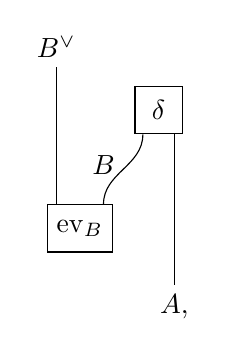
\begin{tikzpicture}[baseline=(current bounding box.center)]
      % Nodes
      \node (Bvee) at (-0.3,3.3) {$B^\vee$};
      \node (deltabox) at (1,2.5) [rectangle, draw, minimum width=0.6cm, minimum height=0.6cm] {$\delta$};
      \node (evbox) at (0,1) [rectangle, draw, minimum width=0.6cm, minimum height=0.6cm] {$\mathrm{ev}_B$};
      \node (A) at (1.2,0) {$A$,};
      \node (B) at (0.3,1.8) {$B$};

      % Edges
      \draw (Bvee) -- (evbox.north -| -0.3,1.3);
      \draw (deltabox.south -| 0.8,2.5) to [out=270,in=90] (evbox.north -| 0.3,1.3);
      \draw (deltabox.south -| 1.2,2.5) -- (A);
    \end{tikzpicture}
  \end{equation*}
  where $B^\vee = \Hom_{\mathcal C}(B,1)$ and $\mathrm{ev}_B\colon B^\vee\otimes B\to 1$ is the evaluation map, i.e. the counit of the adjunction between ${-}\otimes B$ and $\Hom_{\mathcal C}(B,{-})$.
\end{defn}
Let $\Prdual$ denote the category of dualizable stable categories with strongly continuous functors between them. The Lurie tensor product on presentable categories restricts to a symmetric monoidal structure on $\Prdual$. By \cite{Ramzi2024}, this symmetric monoidal structure is closed. We denote the resulting internal mapping object by $\Homd ({-},{-})$.
\begin{defn}[Bartels--Nikolaus]
  Let $\tset$ be a locally compact Hausdorff space. The category of \tdef{completed cosheaves} on $\tset$, denoted $\coShat (\tset )$, is given by
  \[
    \coShat (\tset ) = \Homd (\D{\tset},\Sp ).
  \]
\end{defn}
Although general objects of $\coShat (\tset )$ are quite mysterious, the definition does give us a description of the compact objects via
\[
  \coShat (\tset )^\omega\simeq\Map_{\Prdual}(\Sp ,\coShat (\tset ))
  \simeq\Map_{\Prdual}(\Sp,\Homd (\D{\tset},\Sp ))\simeq\Map_{\Prdual}(\D{\tset},\Sp),
\]
where the final equivalence used the adjunction between internal mapping object and $\otimes$. That is, the groupoid of compact objects $\coShat (\tset )^\omega$ is equivalent to the groupoid strongly continuous functors $\D{\tset}\to\Sp$, which is a subgroupoid of the more familiar groupoid of all colimit-preserving functors $\D{\tset}\to\Sp$. Of particular interest is the strongly continuous functor
\[
\tset_\sharp\colon\D{\tset}\to\Sp
\]
that is left adjoint to $\tset^*$, defined if $\tset$ is locally of singular shape. The corresponding compact object of $\coShat (\tset )$ is denoted $w_\tset$ and referred to as the \tdef{local Wall object} of $\tset$.

Another aspect of $\coShat (\tset )$ which is well-understood by hard work of Bartels--Nikolaus and Efimov is its value under localizing invariants:
\begin{thm}[Bartels--Efimov--Nikolaus]\label{thm: K theory of completed cosheaves}
  $K(\coShat (\tset ))\simeq \tset_*\tset^!K (\SS )$.
\end{thm}
Finally, we will need to introduce some notation for the functoriality of $\coShat (\tset )$. If $h\colon\tset\to\tset '$ is a proper map of locally compact Hausdorff spaces, we get as usual that the pullback $h^*\colon\D{\tset '}\to \D{\tset}$ is strongly continuous. Hence it induces a map on completed cosheaves that we denote
\[
h_?\colon \coShat (\tset )\to \coShat (\tset ').
\]
That is, the category of completed cosheaves is {\em covariantly functorial in proper maps}. Since $h_?$ is strongly continuous by construction, it admits a colimit-preserving left adjoint that we denote
\[
h^?\colon \coShat (\tset ')\to \coShat (\tset ).
\]
The reader may observe that there is an additional contravariant functoriality in etale maps, for instance, that one would might want to denote $h^{\text{?`}}$.


\medskip

Assume that $\tset$ is locally of singular shape and compact. Under these assumptions, we have a sequence of colimit-preserving functors
\[
  \D{\tset}\otimes\Sp^{\fundgroupoid (\tset )}\xrightarrow{\id\otimes\psi^*}
  \D{\tset}\otimes \D{\tset}\xrightarrow{\Delta^*}\D{\tset}\xrightarrow{\tset^*}
  \Sp, 
\]
where $\psi^*\colon \Sp^{\fundgroupoid (\tset )}\to\D{\tset}$ denotes the inclusion of local systems into all sheaves. Bartels and Nikolaus show that the composite $\D{\tset}\otimes\Sp^{\fundgroupoid (\tset )}\to\Sp$ admits a left adjoint
\[
\delta\colon \Sp\to \D{\tset}\otimes\Sp^{\fundgroupoid (\tset )},
\]
which is then a strongly continuous functor and thus a morphism in the category $\Prdual$. Specializing~\cref{defn: abstract assembly} to this situation, we thus get a strongly continuous functor
\begin{equation}
  \label{eq:BN-assembly}
  a_\delta\colon\coShat (\tset )\to \Sp^{\fundgroupoid (\tset )},
\end{equation}
the \tdef{Bartels--Nikolaus assembly functor}.
\begin{thm}[Bartels--Nikolaus]\label{thm: Bartels--Nikolaus geometric topology}
  Let $\tset$ be a compact Hausdorff space that is locally of constant shape.
  Then the functor~\eqref{eq:BN-assembly}
  \begin{enumerate}[label=(\roman*)]
  \item induces the Waldhausen assembly map on $K$-theory and
  \item maps the local Wall object $w_\tset$ to the constant sphere spectrum $\SS_{\fundgroupoid \tset}$.
  \end{enumerate}
\end{thm}
Part (ii) means that we can factor $(\fundgroupoid\tset )^*\colon\Sp\to\Sp^{\fundgroupoid\tset}$ through the Bartels--Nikolaus assembly functor. Better, we have
\begin{prop}
  Let $f\colon \tset\to \tset$ be a self-map of a compact Hausdorff space that is locally of singular shape. Considered as a morphism in $\Endtrl(\Prlstf)$, the lax commutative square~\eqref{eq:lax-comm-square-reidemeister} factors as
  \begin{equation}\label{eq:lax-composition-cosheaves}
\begin{tikzcd}
	\Sp & {\coShat(\tset)} & \Sp^{\ani{\tset}} \\
	\Sp & {\coShat(\tset)} & \Sp^{\ani{\tset}} 
	\arrow["{w_{\tset}}", from=1-1, to=1-2]
	\arrow["\id"', from=1-1, to=2-1]
	\arrow["{a_{\delta}}", from=1-2, to=1-3]
	\arrow["{f^?}", from=1-2, to=2-2]
	\arrow["f^{\ast}", from=1-3, to=2-3]
	\arrow[Rightarrow, from=2-2, to=1-3]
	\arrow["{w_{\tset}}"', from=2-1, to=2-2]
    \arrow[Rightarrow, from=2-1, to=1-2]
	\arrow["{a_{\delta}}"', from=2-2, to=2-3]
\end{tikzcd}
    % \left(
    %   \begin{tikzcd}[column sep=large]
    %     \coShat (\tset ) \arrow[r,"a_\delta"] \arrow[d,"f^?"] & \Sp^{\fundgroupoid (\tset )} \arrow[d,"f^*"]\\
    %     \coShat (\tset ) \arrow[r,swap,"a_\delta"] \arrow[ru,Rightarrow, shorten <=5pt,shorten >=5pt]  & \Sp^{\fundgroupoid (\tset )}
    %   \end{tikzcd}
    % \right)
    % \circ
    % \left(
    %   \begin{tikzcd}[column sep=large]
    %     \Sp \arrow[r,"w_\tset"] \arrow[d,equal] & \coShat (\tset ) \arrow[d,"f^?"]\\
    %     \Sp \arrow[r,swap,"w_\tset"]  \arrow[ru,Rightarrow, shorten <=5pt,shorten >=5pt]  & \coShat (\tset )
    %   \end{tikzcd}
    % \right),
  \end{equation}
  in which the left hand $2$-cell is the transpose of the commutative diagram
  \[
    \begin{tikzcd}[column sep=large]
      \coShat (\tset ) \arrow[r,"a_\delta"] \arrow[d,"f_?"] & \Sp^{\fundgroupoid (\tset )} \arrow[d,"f_!"]\\
      \coShat (\tset ) \arrow[r,swap,"a_\delta"]   & \Sp^{\fundgroupoid (\tset )}
    \end{tikzcd},
  \]
  and the right hand $2$-cell is the transpose of the $2$-cell
  \[
    \begin{tikzcd}[column sep=large]
      \Sp \arrow[r,"w_\tset"] \arrow[d,equal] & \coShat (\tset ) \arrow[d,"f_?"]\\
      \Sp \arrow[r,swap,"w_\tset"]  \arrow[ru,Leftarrow, shorten <=5pt,shorten >=5pt]  & \coShat (\tset )
    \end{tikzcd}
  \]
  coming from the counit transformation
  \[
    f_?(w_\tset) = \tset_\sharp\circ f^*\simeq\tset_\sharp \circ f_\sharp\circ f^*\to\tset_\sharp = w_\tset.
  \]
\end{prop}
\begin{cor}
  Let $f\colon \tset\to \tset$ be a self-map of a compact Hausdorff space that is locally of singular shape. There is a commutative triangle
  \begin{equation}
    \label{eq:nielsen-triangle-without-identification}
    \begin{tikzcd}[column sep=tiny]
      & \tr{f^?\curvearrowright\coShat (\tset )}{}\arrow[dr] \\
      \SS\arrow[rr]\arrow[ru] && \SS\lbrack\cL^{f}\fundgroupoid\tset\rbrack,
    \end{tikzcd}
  \end{equation}
  where the bottom horizontal arrow is the Reidemeister trace.
\end{cor}
\subsection{Another trace ``calculation''}
Keeping with the pattern laid out in~\cref{sec: lefschetz theory}, the next step in our treatment of Lefschetz--Nielsen theory is a calculation of the categorical trace that shows up as the apex in the triangle~\eqref{eq:nielsen-triangle-without-identification}. Unlike in the Lefschetz and Reidemeister trace incarnations of this step, we will not be able to calculate $\tr{f^?\curvearrowright\coShat (\tset )}{}$ in the strict sense (without a big effort); instead, we will give a lax calculation that suffices for the purposes of fixed point theory. This idea is again adapted to our setting from unpublished work of Bartels and Nikolaus, who show using simple manipulations in closed monoidal categories that the map induced on $K$-theory by their assembly functor $a_\delta\colon\coShat (\tset )\to \Sp^{\fundgroupoid (\tset )}$ factors through $\tset_*\tset^!K\SS$, thereby removing the difficult~\cref{thm: K theory of completed cosheaves} from the dependencies of the customer-facing~\cref{thm: Bartels--Nikolaus geometric topology}.

We should expect the calculation of $\tr{f^?\curvearrowright\coShat (\tset )}{}$ to be difficult, because for $f=\id$ it is already a difficult theorem of Efimov.\todo{motivate linearizing over free algebra on dualizable generator}
\begin{defn}[The free algebra on one dualizable object]
  $\freeondual = \Fun (\mathrm{Bord}^1_{\mathrm{fr}}(\RR^1)^{\op},\Sp )$\todo{define Hopf algebra structure}
\end{defn}

